\documentclass[12pt,letterpaper]{article}
\usepackage{graphicx,textcomp}
\usepackage{natbib}
\usepackage{setspace}
\usepackage{fullpage}
\usepackage{color}
\usepackage[reqno]{amsmath}
\usepackage{amsthm}
\usepackage{fancyvrb}
\usepackage{amssymb,enumerate}
\usepackage[all]{xy}
\usepackage{endnotes}
\usepackage{lscape}
\newtheorem{com}{Comment}
\usepackage{float}
\usepackage{hyperref}
\newtheorem{lem} {Lemma}
\newtheorem{prop}{Proposition}
\newtheorem{thm}{Theorem}
\newtheorem{defn}{Definition}
\newtheorem{cor}{Corollary}
\newtheorem{obs}{Observation}
\usepackage[compact]{titlesec}
\usepackage{dcolumn}
\usepackage{tikz}
\usetikzlibrary{arrows}
\usepackage{multirow}
\usepackage{xcolor}
\newcolumntype{.}{D{.}{.}{-1}}
\newcolumntype{d}[1]{D{.}{.}{#1}}
\definecolor{light-gray}{gray}{0.65}
\usepackage{url}
\usepackage{listings}
\usepackage{color}

\definecolor{codegreen}{rgb}{0,0.6,0}
\definecolor{codegray}{rgb}{0.5,0.5,0.5}
\definecolor{codepurple}{rgb}{0.58,0,0.82}
\definecolor{backcolour}{rgb}{0.95,0.95,0.92}

\lstdefinestyle{mystyle}{
	backgroundcolor=\color{backcolour},   
	commentstyle=\color{codegreen},
	keywordstyle=\color{magenta},
	numberstyle=\tiny\color{codegray},
	stringstyle=\color{codepurple},
	basicstyle=\footnotesize,
	breakatwhitespace=false,         
	breaklines=true,                 
	captionpos=b,                    
	keepspaces=true,                 
	numbers=left,                    
	numbersep=5pt,                  
	showspaces=false,                
	showstringspaces=false,
	showtabs=false,                  
	tabsize=2
}
\lstset{style=mystyle}
\newcommand{\Sref}[1]{Section~\ref{#1}}
\newtheorem{hyp}{Hypothesis}

\title{Problem Set 3}
\date{Due: November 13, 2025}
\author{Applied Stats/Quant Methods 1}


\begin{document}
	\maketitle
	\section*{Instructions}
	\begin{itemize}
		\item Please show your work! You may lose points by simply writing in the answer. If the problem requires you to execute commands in \texttt{R}, please include the code you used to get your answers. Please also include the \texttt{.R} file that contains your code. If you are not sure if work needs to be shown for a particular problem, please ask.
	\item Your homework should be submitted electronically on GitHub.
	\item This problem set is due before 23:59 on Thursday November 13, 2025. No late assignments will be accepted.

	\end{itemize}

		\vspace{.25cm}
	
\noindent In this problem set, you will run several regressions and create an add variable plot (see the lecture slides) in \texttt{R} using the \texttt{incumbents\_subset.csv} dataset. Include all of your code.

	\vspace{.5cm}
\section*{Question 1}
\vspace{.25cm}
\noindent We are interested in knowing how the difference in campaign spending between incumbent and challenger affects the incumbent's vote share. 
	\begin{enumerate}
		\item Run a regression where the outcome variable is \texttt{voteshare} and the explanatory variable is \texttt{difflog}.
			\lstinputlisting[language=R, firstline=35, lastline=36]{PS03.R}
			\begin{verbatim}
				Residuals:
				Min       1Q   Median       3Q      Max 
				-0.26832 -0.05345 -0.00377  0.04780  0.32749 
				
				Coefficients:
				Estimate Std. Error t value Pr(>|t|)    
				(Intercept) 0.579031   0.002251  257.19   <2e-16 ***
				difflog     0.041666   0.000968   43.04   <2e-16 ***
				---
				Signif. codes:  0 ‘***’ 0.001 ‘**’ 0.01 ‘*’ 0.05 ‘.’ 0.1 ‘ ’ 1
				
				Residual standard error: 0.07867 on 3191 degrees of freedom
				Multiple R-squared:  0.3673,	Adjusted R-squared:  0.3671 
				F-statistic:  1853 on 1 and 3191 DF,  p-value: < 2.2e-16
			\end{verbatim}
			\textit{A bivariate regression analysis was run by using the lm function in R. A bivariate regression was run because there was an outcome variable, voteshare and one explanatory variable,difflog}
		\item Make a scatterplot of the two variables and add the regression line. 
		\lstinputlisting[language=R, firstline=37, lastline=41]{PS03.R}	
		\textit{I created a scatter plot of the two variables that I would like to observe and also created a regression line through the scatter plot. }
		\begin{center}
			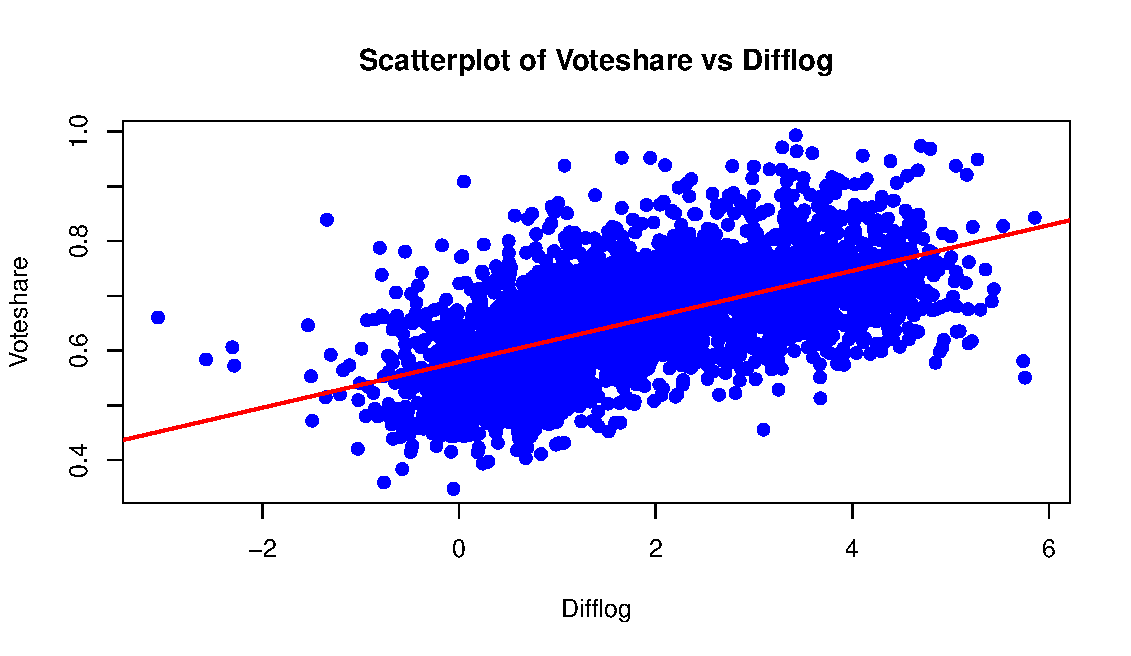
\includegraphics[width=0.7\textwidth]{Voteshare_Difflog.pdf}
		\end{center}
		\item Save the residuals of the model in a separate object.
		\lstinputlisting[language=R, firstline=42, lastline=43]{PS03.R}
			\vspace{7cm}
		\item Write the prediction equation.
		\[
		\widehat{voteshare}_i = \beta_0 + \beta_1 \, difflog_i
		\]
		\[		
		\text{presvote} = 0.579 + 0.0417 \times \text{difflog}
		\]
		
	
			\textit{I used Latex code to do this.}
	\end{enumerate}
	
		
	


\section*{Question 2}
\noindent We are interested in knowing how the difference between incumbent and challenger's spending and the vote share of the presidential candidate of the incumbent's party are related.	\vspace{.25cm}
	\begin{enumerate}
		\item Run a regression where the outcome variable is \texttt{presvote} and the explanatory variable is \texttt{difflog}.
		\lstinputlisting[language=R, firstline=46, lastline=47]{PS03.R}
		\begin{verbatim}
			Residuals:
			Min       1Q   Median       3Q      Max 
			-0.32196 -0.07407 -0.00102  0.07151  0.42743 
			
			Coefficients:
			Estimate Std. Error t value Pr(>|t|)    
			(Intercept) 0.507583   0.003161  160.60   <2e-16 ***
			difflog     0.023837   0.001359   17.54   <2e-16 ***
			---
			Signif. codes:  0 ‘***’ 0.001 ‘**’ 0.01 ‘*’ 0.05 ‘.’ 0.1 ‘ ’ 1
			
			Residual standard error: 0.1104 on 3191 degrees of freedom
			Multiple R-squared:  0.08795,	Adjusted R-squared:  0.08767 
			F-statistic: 307.7 on 1 and 3191 DF,  p-value: < 2.2e-16
		\end{verbatim}
		\textit{A bivariate regression analysis was run by using the lm function in R. A bivariate regression was run because there was an outcome variable, presvote and one explanatory variable,difflog}
			\vspace{5cm}
		\item Make a scatterplot of the two variables and add the regression line. 
		\lstinputlisting[language=R, firstline=48, lastline=52]{PS03.R}	
		
		\textit{I created a scatter plot of the two variables that I would like to observe and also created a regression line through the scatter plot. }
			\begin{center}
			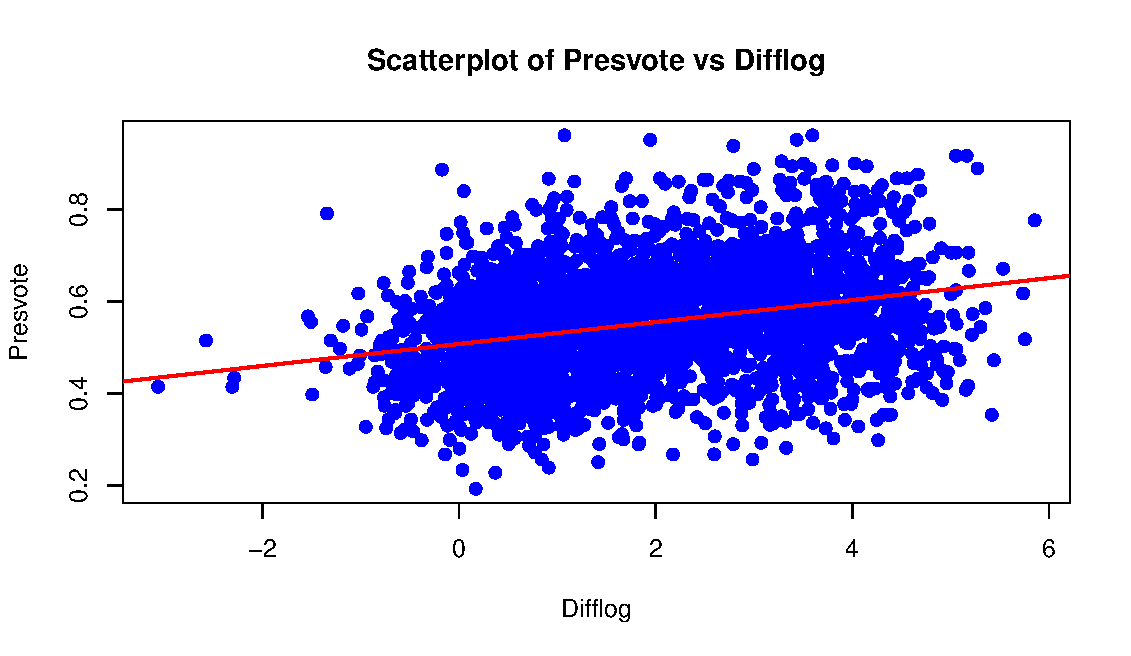
\includegraphics[width=0.7\textwidth]{presvote_difflog.pdf}
		\end{center}
			\vspace{5cm}
		\item Save the residuals of the model in a separate object.
		\lstinputlisting[language=R, firstline=53, lastline=54]{PS03.R}
			\vspace{5cm}
		\item Write the prediction equation.
		\[
		\widehat{presvote}_i = \beta_0 + \beta_1 \, difflog_i
		\]
		\[
		\text{presvote} = 0.507583 + 0.023837 \times \text{difflog}
		\]
		\textit{I used Latex code to do this.}
	\end{enumerate}
	
	\newpage	
\section*{Question 3}

\noindent We are interested in knowing how the vote share of the presidential candidate of the incumbent's party is associated with the incumbent's electoral success.
	\vspace{.25cm}
	\begin{enumerate}
		\item Run a regression where the outcome variable is \texttt{voteshare} and the explanatory variable is \texttt{presvote}.
			\lstinputlisting[language=R, firstline=58, lastline=59]{PS03.R}
			\begin{verbatim}
				Residuals:
				Min       1Q   Median       3Q      Max 
				-0.27330 -0.05888  0.00394  0.06148  0.41365 
				
				Coefficients:
				Estimate Std. Error t value Pr(>|t|)    
				(Intercept) 0.441330   0.007599   58.08   <2e-16 ***
				presvote    0.388018   0.013493   28.76   <2e-16 ***
				---
				Signif. codes:  0 ‘***’ 0.001 ‘**’ 0.01 ‘*’ 0.05 ‘.’ 0.1 ‘ ’ 1
				
				Residual standard error: 0.08815 on 3191 degrees of freedom
				Multiple R-squared:  0.2058,	Adjusted R-squared:  0.2056 
				F-statistic:   827 on 1 and 3191 DF,  p-value: < 2.2e-16
			\end{verbatim}
			\textit{A bivariate regression analysis was run by using the lm function in R. A bivariate regression was run because there was an outcome variable, voteshare and one explanatory variable,presvote}
			\vspace{5cm}
		\item Make a scatterplot of the two variables and add the regression line.
			\lstinputlisting[language=R, firstline=60, lastline=66]{PS03.R}
			\textit{I created a scatter plot of the two variables that I would like to observe and also created a regression line through the scatter plot. } 
				\begin{center}
				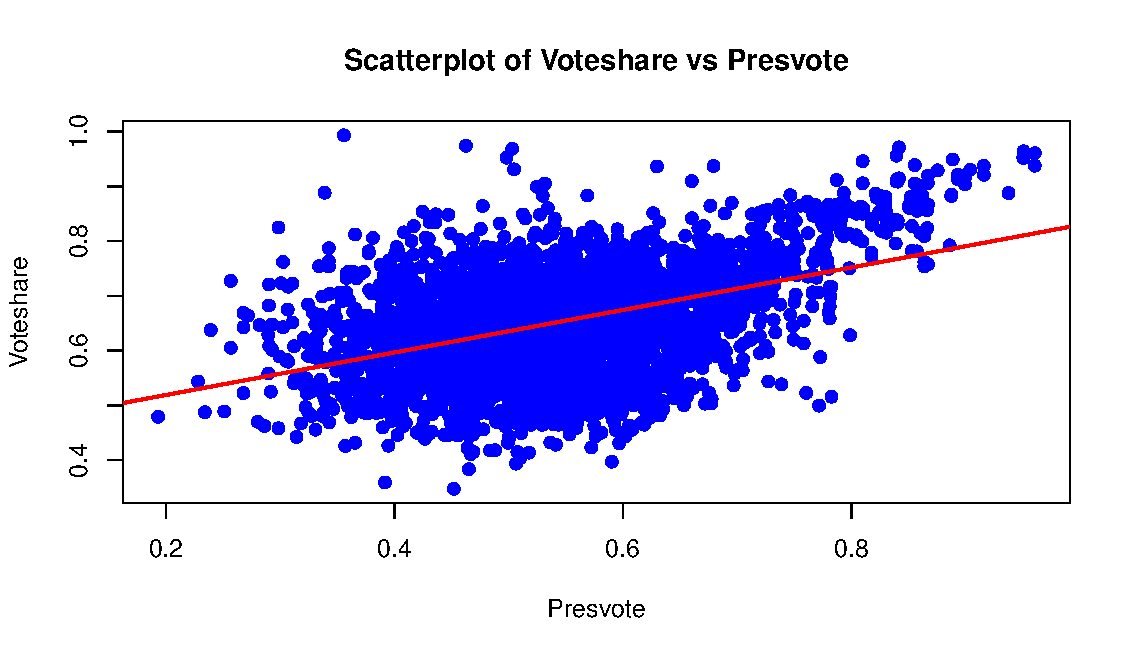
\includegraphics[width=0.7\textwidth]{voteshare_presvote.pdf}
			\end{center}
			\vspace{5cm}
		\item Write the prediction equation.
		\[
		\widehat{voteshare}_i = \beta_0 + \beta_1 \, presvote_i
		\]
		\[
		\text{voteshare} = 0.441330 + 0.388018 \times \text{presvote}
		\]
			\textit{I used Latex code to do this.}
	\end{enumerate}
	

\newpage	
\section*{Question 4}
\noindent The residuals from part (a) tell us how much of the variation in \texttt{voteshare} is $not$ explained by the difference in spending between incumbent and challenger. The residuals in part (b) tell us how much of the variation in \texttt{presvote} is $not$ explained by the difference in spending between incumbent and challenger in the district.
	\begin{enumerate}
		\item Run a regression where the outcome variable is the residuals from Question 1 and the explanatory variable is the residuals from Question 2.
			\lstinputlisting[language=R, firstline=72, lastline=73]{PS03.R}
			\begin{verbatim}
				Residuals:
				Min       1Q   Median       3Q      Max 
				-0.25928 -0.04737 -0.00121  0.04618  0.33126 
				
				Coefficients:
				Estimate Std. Error t value Pr(>|t|)    
				(Intercept)       -5.934e-18  1.299e-03    0.00        1    
				residuals_model_2  2.569e-01  1.176e-02   21.84   <2e-16 ***
				---
				Signif. codes:  0 ‘***’ 0.001 ‘**’ 0.01 ‘*’ 0.05 ‘.’ 0.1 ‘ ’ 1
				
				Residual standard error: 0.07338 on 3191 degrees of freedom
				Multiple R-squared:   0.13,	Adjusted R-squared:  0.1298 
				F-statistic:   477 on 1 and 3191 DF,  p-value: < 2.2e-16
				
				>
			\end{verbatim}
			\textit{A bivariate regression analysis was run by using the lm function in R. A bivariate regression was run because there was an outcome variable, residuals from question 1 and one explanatory variable,the residuals from Question 2.}
			\vspace{6cm}
		\item Make a scatterplot of the two residuals and add the regression line.
		\textit{I created a scatter plot of the two variables that I would like to observe and also created a regression line through the scatter plot. }  
			\lstinputlisting[language=R, firstline=75, lastline=81]{PS03.R}
				\begin{center}
				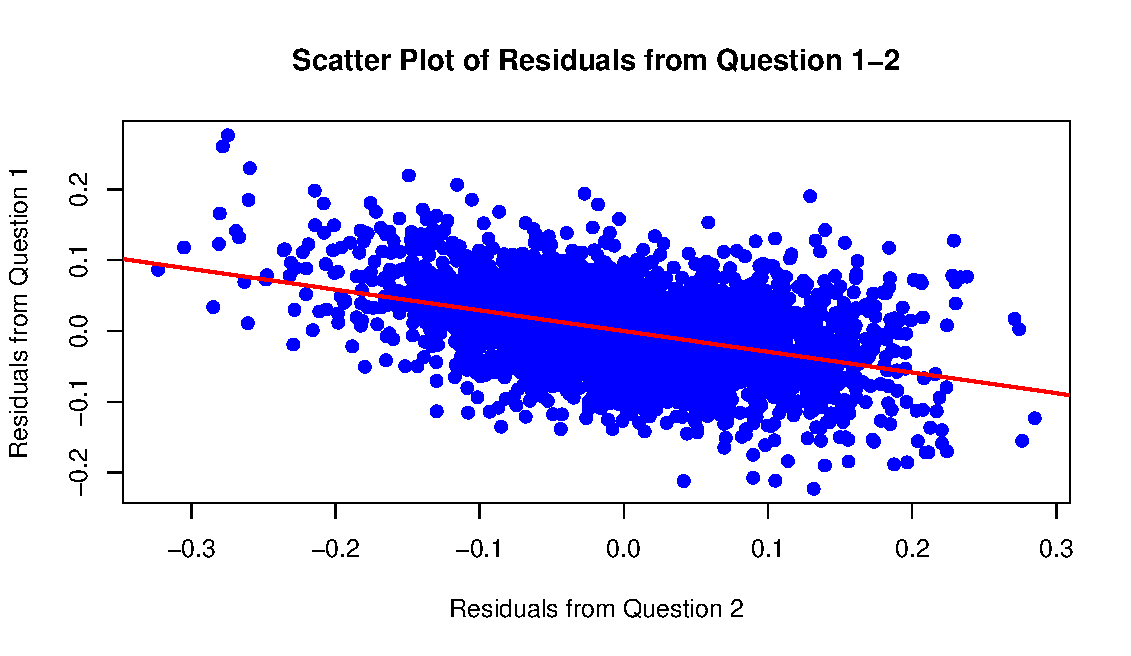
\includegraphics[width=0.7\textwidth]{residuals.pdf}
			\end{center}
			\vspace{6cm}
		\item Write the prediction equation.
		\begin{equation*}
			\hat{\text{residuals1}} = \beta_0 + \beta_1 \cdot \text{residuals2}
		\end{equation*}
	\end{enumerate}
	\[
	\text{residuals\_model\_1} = -5.934 \times 10^{-18} + 0.2569 \times \text{residuals\_model\_2}
	\]
	
	\newpage	

\section*{Question 5}
\noindent What if the incumbent's vote share is affected by both the president's popularity and the difference in spending between incumbent and challenger? 
	\begin{enumerate}
		\item Run a regression where the outcome variable is the incumbent's \texttt{voteshare} and the explanatory variables are \texttt{difflog} and \texttt{presvote}.
			\lstinputlisting[language=R, firstline=83, lastline=84]{PS03.R}	
			\begin{verbatim}
			Residuals:
			Min       1Q   Median       3Q      Max 
			-0.25928 -0.04737 -0.00121  0.04618  0.33126 
			
			Coefficients:
			Estimate Std. Error t value Pr(>|t|)    
			(Intercept) 0.4486442  0.0063297   70.88   <2e-16 ***
			difflog     0.0355431  0.0009455   37.59   <2e-16 ***
			presvote    0.2568770  0.0117637   21.84   <2e-16 ***
			---
			Signif. codes:  0 ‘***’ 0.001 ‘**’ 0.01 ‘*’ 0.05 ‘.’ 0.1 ‘ ’ 1
			
			Residual standard error: 0.07339 on 3190 degrees of freedom
			Multiple R-squared:  0.4496,	Adjusted R-squared:  0.4493 
			F-statistic:  1303 on 2 and 3190 DF,  p-value: < 2.2e-16
		\end{verbatim}
				\textit{This is a multivariate regression where multiple explanatory variables (difflog and presvote) are being compared against one outcome variable, vote share.I changed the regression analysis in R to reflect this.}
			\vspace{5cm}
		\item Write the prediction equation.
			
		\textit{For a multivariate analysis you include multiple variables in the equation.}
		\begin{equation}
			\begin{aligned}
				\hat{\text{voteshare}} =\ & \beta_0 + \beta_1 \cdot \text{difflog} + \beta_2 \cdot \text{presvote} 
			\end{aligned}
		\end{equation}
		\[
		\text{voteshare} = 0.4486442 + 0.0355431 \times \text{difflog} + 0.2568770 \times \text{presvote}
		\]	\vspace{5cm}
		\item What is it in this output that is identical to the output in Question 4? Why do you think this is the case?
		
			\textit{The coefficient for the residual 2 is identical to the presvote coefficient. This value is 0.2568. This is because of the Frisch-Waugh-Lovell Theorem that states that the coefficient for a variable in a multivariate regression will be the same as a coefficient you would get from a two step process. In this problem set, I did a two step process where I regressed the dependent variable on the independent variable and then took the residual of that  }
	\end{enumerate}




\end{document}
